Let's suppose now we have no feeling at all for theoretical optimality
guarantees, we just want to obtain a solution as fast as possible and,
hopefully, a good one. That's when the \emph{heuristic} approaches take place:
they're fast algorithms (typically polynomial) and in some cases, on average,
they're close to the optimal solution for no more than 2-3\%. Again, there's no
theoretical guarantee on the worse case, but in practice they work pretty well.

We can split heuristic approaches into two subcategories:
\begin{itemize}
    \item \emph{Constructive heuristics}: they built a solution from scratch
    \item \emph{Refinement heuristics}: starts with a solution while iteratively
        improving it. Hard and Soft Fixing are examples of this category
\end{itemize}

\section{Constructive Heuristics}

\subsection{Greedy}
The first constructive heuristic we're going to present follows a \emph{greedy}
strategy to solve TSP: sitting in a node, the next one in the path will be the
one at the shortest distance or, if there are no other nodes to visit, the tour
returns to the starting node. The approach follows the greedy paradigm
because at each node it selects the best local solution, i.e., the closest
node.\\
Excluding the starting node and the last one (that closes the loop), we have to
repeat the process $n -2$ times (let's say $\mathcal{O}(n)$) in which we have to
select the next node among $\mathcal{O}(n)$ possibilities. The algorithm runs in
$\mathcal{O}(n^2)$, which is pretty fast compared to a MIP solver. For that
reason, it's possible to repeat the greedy process for each node and finally
select the best tour among all solutions by raising the computational complexity 
to $\mathcal{O}(n^3)$, which remains fast enough.\\

An important thing to notice is that the algorithm is fully  deterministic,
there's no room for parameter tuning or different strategies. If one would
impose a time limit on this method, it could simply stop the computation and
keep the best solution found until the stop.

\subsection{GRASP}
To spice things up, one could extend the greedy paradigm by injecting randomness
into the process. One possibility is to randomize the greedy choice among the best
$k$ options one may have while selecting the next node. This introduces
variability and, in the long run, this approach produces better results. Another
thing that is possible to randomize is the initial choice of the starting
node. We will refer to this as \emph{GRASP: Greedy randomized adaptive search procedure}\\
The approach runs in $\mathcal{O}(n^2)$ for starts, but since the randomness in
the tour and the randomness of the starting node, this approach could run
indefinitely. It will search among a subset of the (finite) possible subtours
according to the greedy choice. For this reason, this approach will run until a
time limit is reached.

\subsubsection{Implementation details}
The greedy approach implementation is straightforward.\\ 
For the grasp approach, a data structure that maintains the top-$k$ choices is
implemented as a priority queue that is implemented as a max binary heap of
fixed $k$ elements. Notice that, even if we're searching for the
shortest-distances node (so we have to minimize the distances in our data
structure), we're only interested in fast retrieval of the distance of the
$k$-th node. In this way, one could pop out that node if a shorter distance
node is encountered. Then, one of the $k$ nodes in the pool can be randomly
chosen.

\subsection{Extra Mileage}
Another constructive heuristic is based on a simple move that builds a solution
starting from a subtour. Suppose that we want to add node $x$ to the tour,
ideally, we're going to break the closest edge $\{a, b\}$ to that node and add
two new edges, $\{a, x\}$ and $\{x, b\}$ so the new node is included. This is
called \emph{extra mileage move}, because among all the possible edges already
included in the tour and all the nodes not included (suppose that we want to
search also the best $x$) it's ideal to perform a move on the ones that
minimize the \emph{extra mileage} $\Delta_{\{a,b\},x} = c(a,x) + c(x, b) - c(a,
b)$. We will repeat this move until a tour has been formed.

\begin{figure}[h]
    \centering
    \begin{minipage}{.33\textwidth}
        \centering
        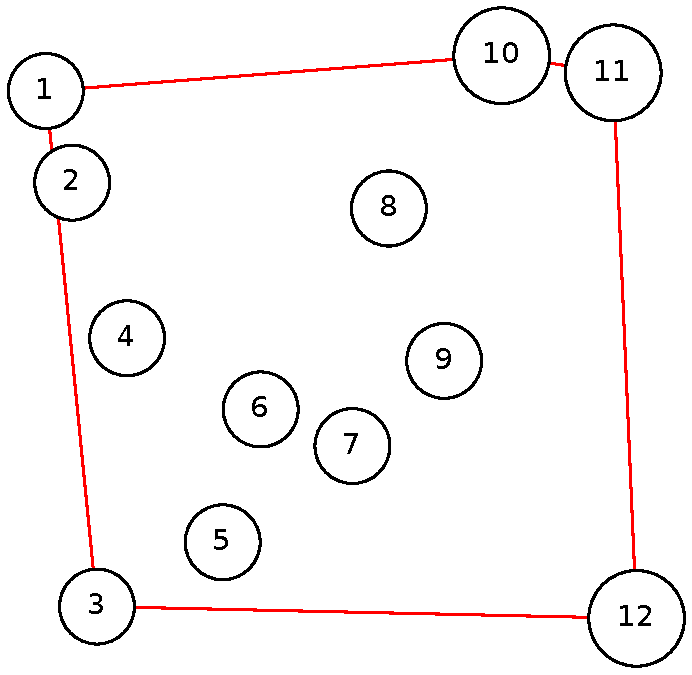
\includegraphics[width=0.8\linewidth]{figures/heura}
        \label{fig:sub1}
    \end{minipage}%
    \begin{minipage}{.33\textwidth}
        \centering
        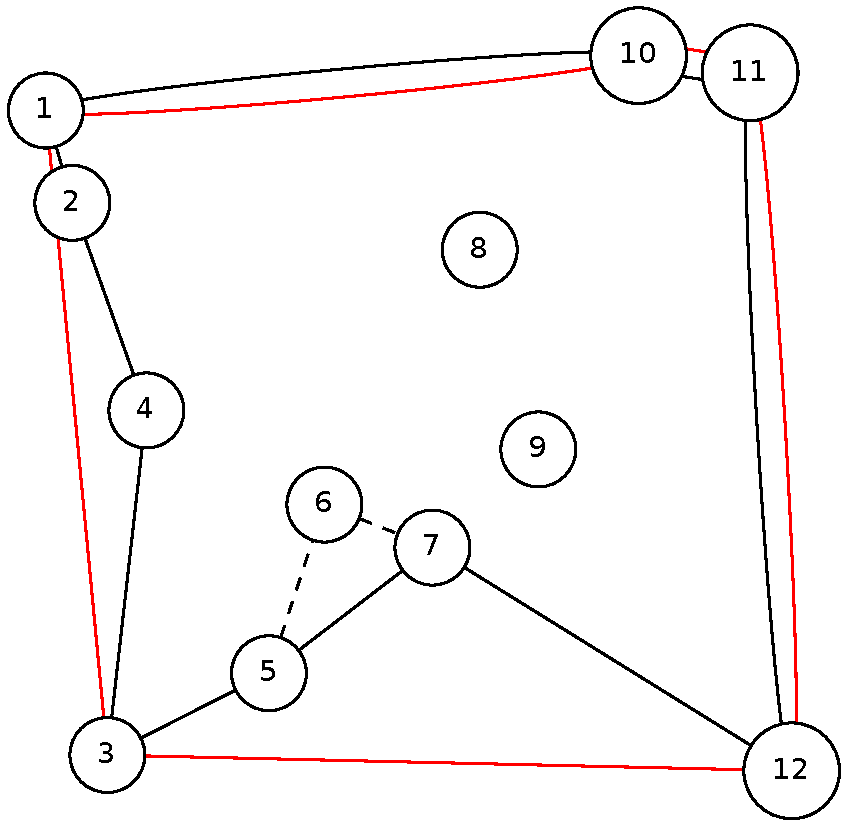
\includegraphics[width=0.8\linewidth]{figures/heurb}
        \label{fig:sub2}
    \end{minipage}
    \begin{minipage}{.33\textwidth}
        \centering
        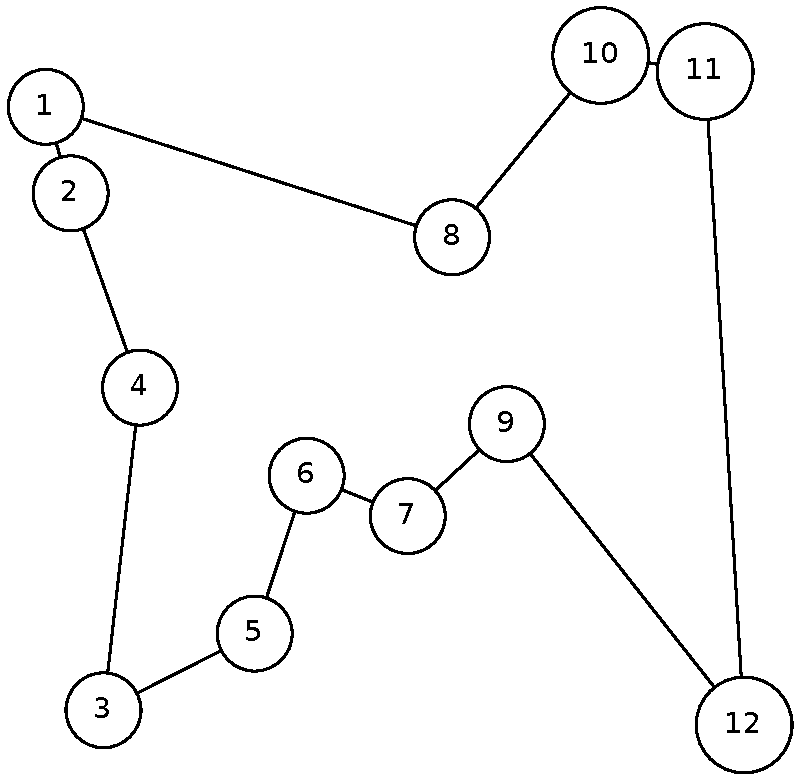
\includegraphics[width=0.8\linewidth]{figures/heurc}
        \label{fig:sub2}
    \end{minipage}
    \caption{\centering Extra mileage algorithm starting from convex hull}
\end{figure}

Since selecting an edge and a node that minimizes the extra mileage will take
$\mathcal{O}(n^2)$, and since we have $\mathcal{O}(n)$ nodes to include in the
tour, the algorithm runs in $\mathcal{O}(n^3)$. The algorithm, as greedy, is
fully deterministic.\\
There's multiple ways to select an initial subtour, in principle, any could work.
Anyway, there are two preferred choices: starts from a subtour of the two most
distant nodes or starts from the frontier of the convex hull, the unique and
smallest set that encloses all the nodes.

\subsubsection{Implementation details}
The implementation is straightforward. It has been selected to start from the
convex hull of the nodes, computed with a popular Graham's scan variant:
Andrew's Monotone chain algorithm, bases on counter-clockwise turn substructure
property that runs on $\mathcal{O}(nlogn)$, anyway absorbed in the
$\mathcal{O}(n^3)$ total complexity.

\subsection{Constructive heuristics comparison}

\begin{claim}
    Extra milage and greedy are good algorithms, leaving aside the computational
    cost. GRASP have the same performance as greedy. 2-approx, despite the
    guarantees, is not a good algorithm.
\end{claim}

\begin{figure}[h]
    \centering
    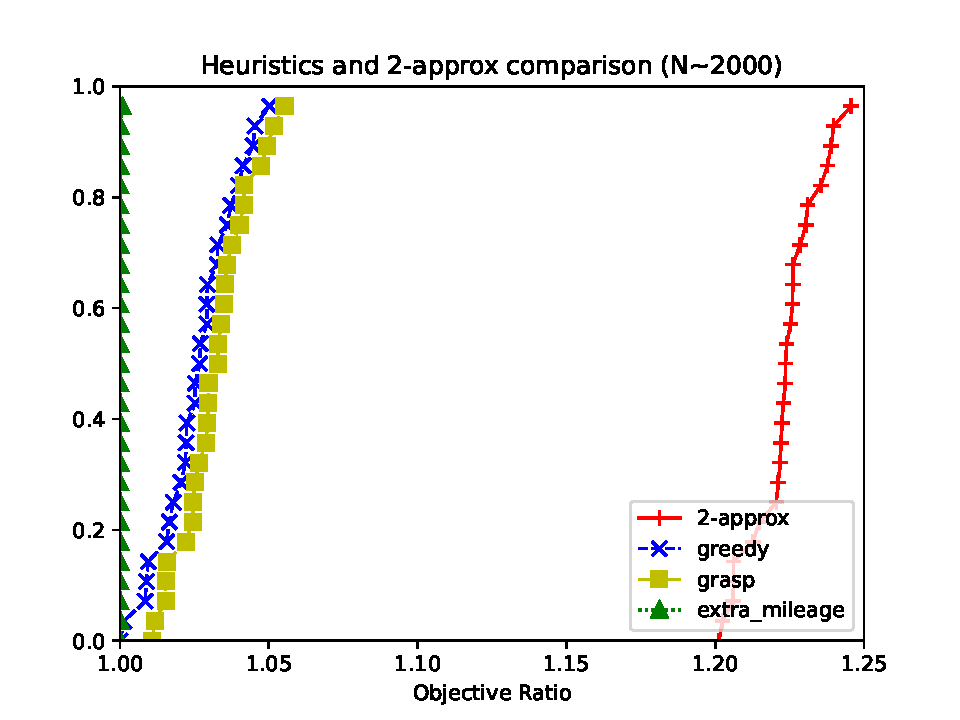
\includegraphics[width=0.8\textwidth]{figures/heuristic_firstcomp}
    \caption{heuristics and 2-approx comparison}
\end{figure}

A first comparison has been done on 30 instances of 2000 nodes each. The graph
presented has the same meaning as the previous ones, except that
the objective function is considered instead of times. The number of nodes has
been chosen to let the $\mathcal{O}(n^3)$ algorithms run in a reasonable amount
of time by letting them reach convergence. \\
The winner is Extra Mileage algorithm, which has the same
complexity as greedy, both achieves good results. The main difference between
these approaches is that greedy's results are the best results among various
runs of the algorithm (by considering different starting nodes) while extra
mileage just produces one result. This can be a huge disadvantage considering
that it's not possible to set a time limit at all: while greedy even if stopped
will produce some good results, extra mileage will not, and time limit
management will be crucial in future approaches. \\
GRASP can be considered as good as greedy, even more flexible because of
randomness. In this test, grasp seems to achieve worse results compared with
greedy and this can be due caused by two factors: a sub-optimal tuning of $k$
(set to $5$) and especially the time limit management. Even if we compared
different algorithms with different behaviors, a common time limit has been
chosen to let the $\mathcal{O}(n^3)$ converge (especially extra-mileage
that will produce only one result). In this settings, also greedy will converge
and that means that the algorithm has explored all possible starting nodes, but
that will not happen with bigger instances, when even if let run for a
reasonable amount of time, the algorithm will explore only a small subset of all
possible starting nodes. And that's when grasp's randomness will become
competitive.\\ 
Recalling that it belongs in a different category, 2-approx's performances are not
exciting, even it's very fast: it produces just one result as extra mileage, and
it's not tunable at all. There's no room for improvement.

\section{Refinement heuristics}

Even without theoretical guarantees, a heuristic is considered decent if it
reaches 5\% from optimality, while the most sophisticated ones  can reach <1\%.
The constructive heuristics we presented, unfortunately, will not easily reach
those results: they will need refinement. \\
Refinement heuristics, applied to an initial yet feasible solution, will improve
the results by exploiting a simple property of euclidean distance.

\subsection{$k$-opt moves}

In $\Delta$-TSP (but also in Euclidean TSP since it's a particular case) the
costs must respect with triangular inequality $c_{ij} \leq c_{ik} + c_{kj},\
\forall\ i, j, k$. By keeping in mind this  property and since we're mainly
working in the case where nodes are 2D coordinates-located cities, a solution
can be improved if a \emph{crossing} is detected. The reason is that, by
triangular inequality applied to the triangle that forms with the center of
the crossing, it's always possible to reach the city $c$ from $a$ directly instead
of reaching it by moving first into another one $b$ and then follow
that leads to $c$.\\
This crossing-deletion procedure is the main idea behind \emph{$k$-moves}:
when a crossing is detected it is deleted, and instead of it two new arcs will be
added. This particular case where the arcs involved are two is called $2$-move.
It's possible to generalize to $k$-move: a rearrangement of $k$ arcs in a way to
reduce the cost of the solution.\\

Considering $x^H$ the current solution, $k$-opt moves can be interpreted in another
way. A move defines a translation of $x^H_0$ in the solution space within a
neighborhood as large as $k$ improves. By rearranging a huge amount of arcs,
there's a lot of room for improvement and so the neighborhood is larger. This is
the same interpretation as we did in Chapter \ref{chap:Matheuristics}. After
a move has  been applied, the new current solution $x^H_1$ is centered is
another neighborhood and the process is repeated until the solution cannot be
improved no more, stuck in a \emph{local optima}. The entire process can be
repeated considering another fresh new solution $x^H_0$. We will refer to this
as \emph{multi-start}, that can be repeated until a time limit is reached.

\subsubsection{$2$-opt moves}
Let's focus on $2$-opt moves. We're still considering the symmetric formulation of
the problem, but let's move to the asymmetric one for simplicity (that's why
before we talked about arcs and not edges). Suppose we found a crossing between
arcs $a \rightarrow b$ and $c \rightarrow d$. The move can be summarized in this
way: remove the arcs $a \rightarrow b$ and $c \rightarrow d$, add $a \rightarrow
c$ and $b \rightarrow d$, and, because the solution has to remain feasible,
reverse the path $b \leadsto c$.

\begin{figure}[h]
    \centering
    \begin{minipage}{.45\textwidth}
        \centering
        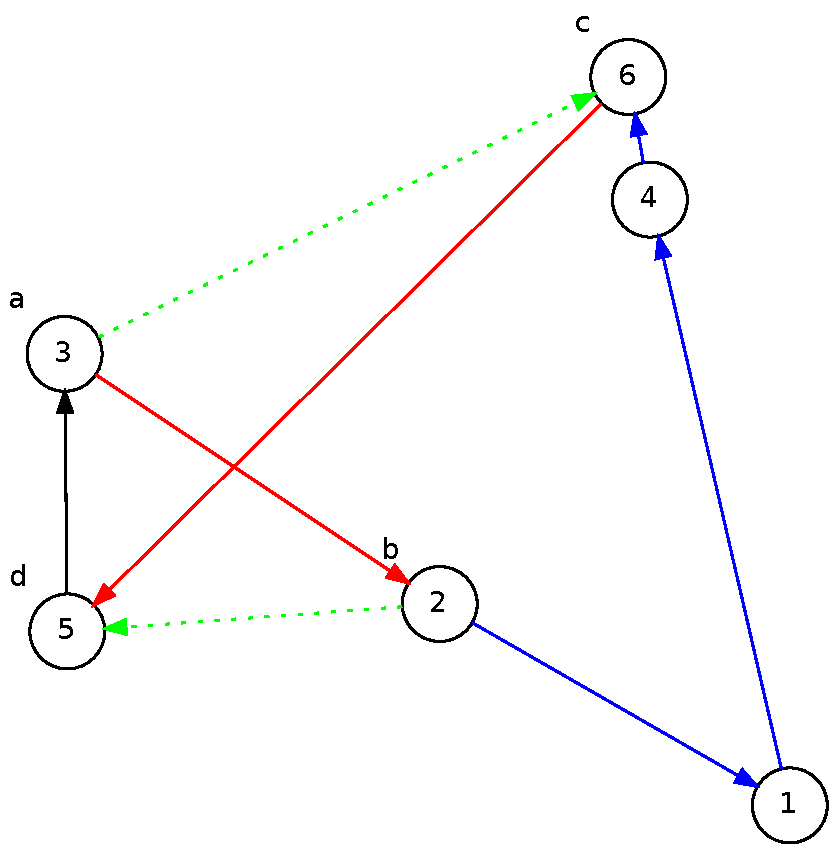
\includegraphics[width=0.8\linewidth]{figures/2move_before.pdf}
    \end{minipage}%
    \begin{minipage}{.45\textwidth}
        \centering
        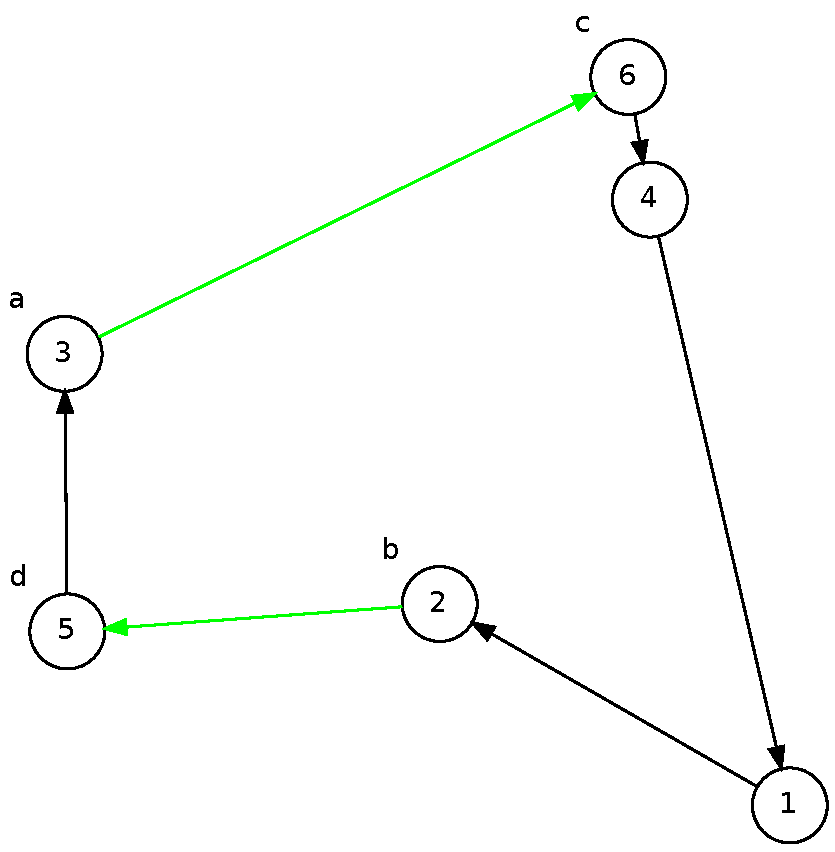
\includegraphics[width=0.8\linewidth]{figures/2move_after.pdf}
    \end{minipage}
    \caption[$2$-opt move example]{\centering $2$-opt move example: red arcs needs to be deleted, green
    to be added and there's the blue path to reverse}
\end{figure}

While it's possible to reverse a huge number of arcs ($\mathcal{O}(n)$), it's in
practice a very fast operation.\\
The last thing to do is a crossing-detection algorithm. There exists a
computational geometry sliding window-based algorithm, but since we're working
with costs it's possible to detect a crossing by analyzing the following value:

\begin{equation}
    \Delta(a,c) = c_{a,c} + c_{b,d} - [c_{a,b} + c_{c,d}]
\end{equation}

This corresponds to the difference between the objective function of the new
tour minus the old one, after a move that involves nodes $a$ and $c$. Notice
that even if we're working on the asymmetric formulation since we started from
a symmetric one, the reversed path has the same cost as the original one, and it
does not matters in the formula. If $\Delta < 0$ there's a crossing and a $2$-move can
be applied.\\
Among all the possible moves that can be applied to a solution $x^H_k$, one
may choose the one with minimum delta or just the first one that encounters.
Since a move is applied starting from a pair of nodes (and their successors),
one may possible to search among $\mathcal{O}(n^2)$ possible moves to find the
one with minimum delta, which sounds fair because the computation of $\Delta$
and the move are cheap operations.

\subsubsection{$3$-opt moves}
After a solution has been refined with all possible $2$-opt moves it becames
crossing-free, but there's still room for improvement. One thing that is
possible to do is to enlarge the neighborhood size by considering $3$-opt moves to
search for better solutions.  Now the thing starts to become complicated
because, to search for minimum $\Delta$, we have to search among
$\mathcal{O}(n^3)$ triplets of nodes and as opposed to previous case, among a
single triplets there's multiple way to reconnect the arcs, and so multiple way
to compute $\Delta$. Both searching and reconnecting are more costly.\\ 
For this reason, usually, this kind of refinement heuristics are implemented so
multiple cheap operations are preferred to few, costly, ones. And so $2$-opt moves
and $3$-opt moves are preferred over $k$-opt moves with $k$ elevated, since it will run
in $\mathcal{O}(n^k)$

\subsection{Implementation details}
Multi-start refinements with moves lead to lots of possibilities in terms of
tuning, that take shape in form of time limit management. The first, obvious,
thing to test is how far we can move in term of neighborhood size. In case of
$3$-opt moves, after the generation of a starting solution (using GRASP), we're
going to apply as many moves as possible, followed by as many $2$-opt moves as
possible. If we want to restrict on $2$-opt moves only, we can clearly skip the
application of $3$-opt moves. If during one of this processes the computation
reaches time limit, the computation for that start is stopped and the best
solution among all starts (also considering the actual partial one) is
returned.\\ One thing that one could may ask is if is more clever to allow more
starts (and so keeping the computation light, maybe skipping $3$-opt moves) or
bet on few, more optimized but heavy, computations.

\begin{claim}
    Skipping $3$-opt moves and allowing more starts is a good idea.
\end{claim}

\begin{figure}[h!]
    \centering
    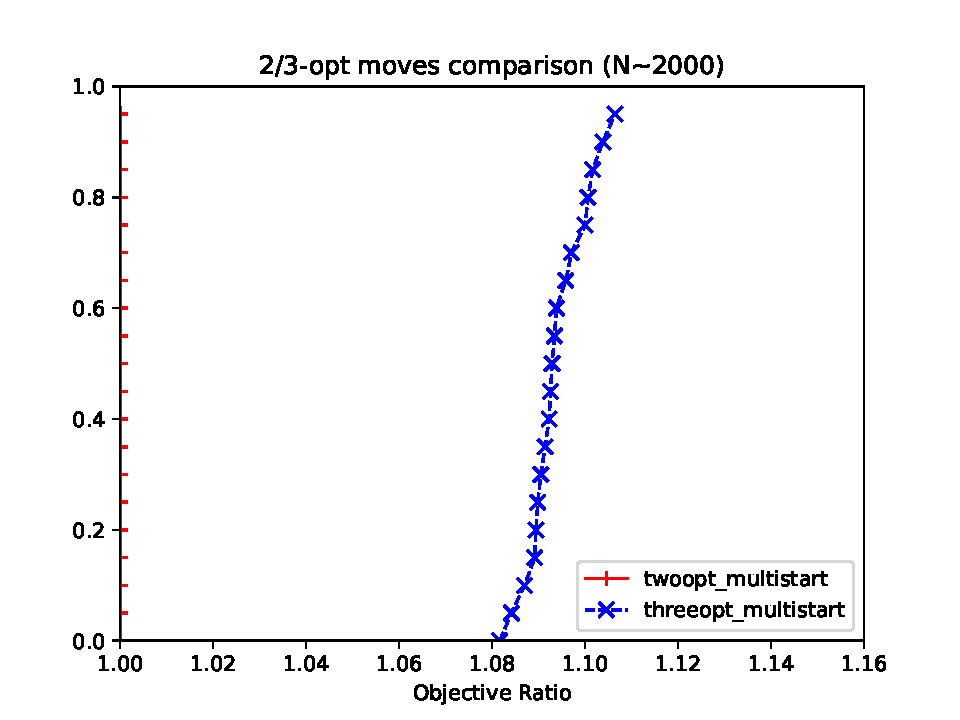
\includegraphics[width=0.7\textwidth]{figures/twothree}
    \caption{Comparison between $2$-opt and $3$-opt moves multi start}
\end{figure}

Our tests on 20 instances of 2000 nodes each shows (even if it's difficult to
visualize) that skipping $3$-opt moves is a good idea. In practice, in the
majority of executions, while with $2$-opt moves only there's multiple restarts,
that allows to pick a good solution, the computat stops before all the
possible $3$-opt moves can be found and applied, so it stuck on the first start.
Actually only few of them are applied and, even if the objective improves a lot,
this approach is worse than apply lots of small improvement.\\

Let's now focus on the initial solution generation. As stated before, GRASP is
used for the process, but one could choose to let internally run GRASP for a
greater amount of time in order to obtain a better inintial solution, that means
few crossing to fix and more multiple starts to perform in the same time limit.
Is it worth spending more initial time on GRASP?

\begin{claim}
    A better initial solution is preferred in multi start approach.
\end{claim}

\begin{figure}[h]
    \centering
    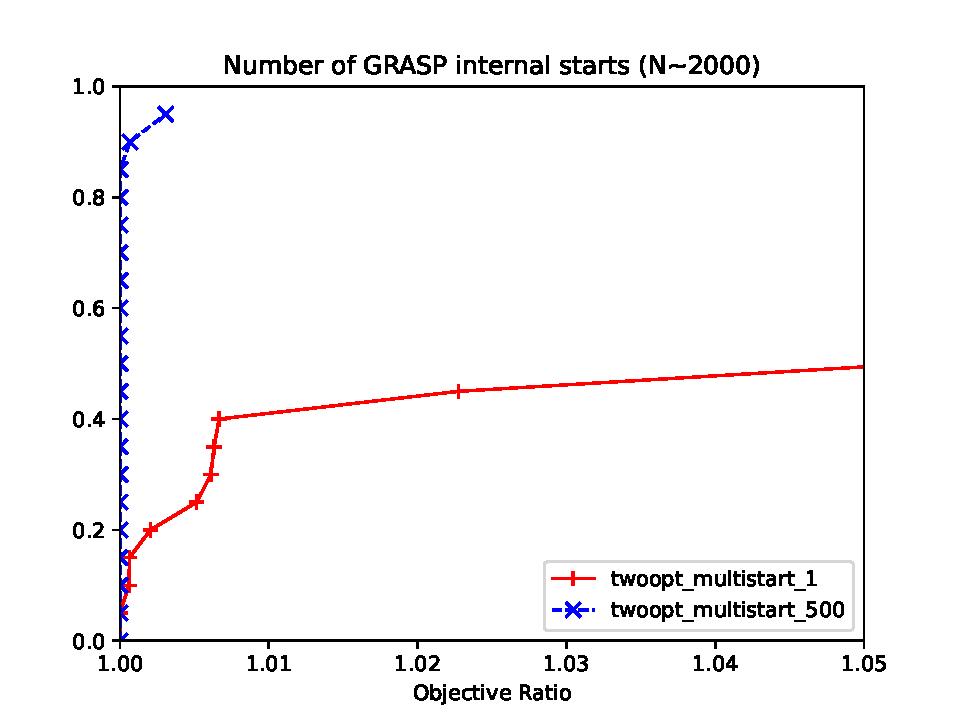
\includegraphics[width=0.8\textwidth]{figures/grasp_starts.pdf}
    \caption{$2$-opt moves multistarts on different GRASP internal starts}
\end{figure}

We tested 20 instances of 2000 nodes each, where the comparison is between
$2$-opt moves refinements considering two scenario for the initial starting
solution $x^H_0$: the first one found by GRASP and the best among 500 starts of
the constructive heuristic, a huge amount considering that is $\nicefrac{1}{4}$
of the total number of nodes. The initial computational cost is clearly higher
but, since it's a better solution, it presents fewer number of crosses and so
the $2$-opt refinement will take less time, (since it's the most costly
operation within a start). The best objective improves, as it can be seen in the
graph, for a single start (because it starts from a better solution) and in
general because, with the time saved, more starts are possible, which doubles.
Since we notices a bit of variability of refined solutions in different starts,
this can only be beneficial.
